\documentclass{article}
\usepackage[utf8]{inputenc}
\usepackage[letterpaper, portrait, margin=1in]{geometry}
\usepackage{enumerate}
% Display only levels as deep as subsection in tableofcontents
\setcounter{tocdepth}{2}

\usepackage{caption}
\usepackage{graphicx}
\graphicspath{ {images/} }
\usepackage{array}

\usepackage{tikz}
\usepackage{verbatim}
\usetikzlibrary{positioning,arrows,shapes}

\usepackage{multirow,booktabs}

% Define function subcommands
\newcommand{\name}[1]{\hline \multicolumn{2}{|l|}{\texttt{#1}} }
\newcommand{\inp}[1]{\hline \textbf{Input:} & #1}
\newcommand{\out}[1]{\hline \textbf{Output:} & #1}
\newcommand{\desc}[1]{\hline \textbf{Description:} & #1 }

% Define function command
\newcommand{\fcn}[4]{
    \begin{center}
    \begin{tabular}{|p{2cm} p{10cm}|}
    \hline
    \name{#1} \\
    \inp{#2} \\
    \out{#3} \\
    \desc{#4} \\
    \hline
    \end{tabular}
    \end{center}
}

% Define function for image table 


%%%%%%%%%%%%%%%%%%%%%%%%%%%%%%%%%%%%%%%%%%%%%%%%%%%
% HEADER
%%%%%%%%%%%%%%%%%%%%%%%%%%%%%%%%%%%%%%%%%%%%%%%%%%%
\usepackage{fancyhdr}
\pagestyle{fancy}
\fancyhf{}
\fancyhead[C]{PiSonal Trainer: Weight Lifting Performance Tracker}
\fancyfoot[L]{Detailed Design}
\fancyfoot[R]{\thepage}
\renewcommand{\headrulewidth}{0.4pt}
\renewcommand{\footrulewidth}{0.4pt}

% Use this to pad tables
\usepackage{array}
\setlength\extrarowheight{6pt}

% Define tab command
\newcommand\tab{\hspace*{2cm}}


%%%%%%%%%%%%%%%%%%%%%%%%%%%%%%%%%%%%%%%%%%%%%%%%%%%
% TITLE
%%%%%%%%%%%%%%%%%%%%%%%%%%%%%%%%%%%%%%%%%%%%%%%%%%%
\title{
PiSonal Trainer: Weight Lifting Performance Tracker\\
\Large {Detailed Design}
}
\date{April 1, 2017}
\author{Birunthaa Umamahesan \and Micaela Estabillo \and Simarpreet Singh}

\begin{document}
%%%%%%%%%%%%%%%%%%%%%%%%%%%%%%%%%%%%%%%%%%%%%%%%%%%
% COVER PAGE
%%%%%%%%%%%%%%%%%%%%%%%%%%%%%%%%%%%%%%%%%%%%%%%%%%%
\thispagestyle{plain}
\pagenumbering{gobble}
\maketitle
\vfill
\begin{center}
    Prepared for Computer Science 4ZP6: Capstone Project \\
    Instructor: Dr. Wenbo He
    Fall/Winter 2016-2017\\
\end{center}
\newpage

%%%%%%%%%%%%%%%%%%%%%%%%%%%%%%%%%%%%%%%%%%%%%%%%%%%
% TABLE OF CONTENTS AND REVISION HISTORY
%%%%%%%%%%%%%%%%%%%%%%%%%%%%%%%%%%%%%%%%%%%%%%%%%%%
\tableofcontents

\listoffigures

\listoftables

\thispagestyle{plain}
\pagenumbering{gobble}

\newpage

\section*{Revision History}
\begingroup
\begin{tabular}{ | p{2cm} | p{1.5cm} | p{3.8cm} | p{7cm} |} 
    \hline
    \textbf{Date} & \textbf{Version} & \textbf{Primary Author} & \textbf{Comment}\\
    \hline
    04/01/2017 & 1.00 & Birunthaa Umamahesan & Final  editing and proofreading for revision 1\\ 
    \hline
    04/01/2017 & 1.00 & Micaela Estabillo & Adjust technical specifications based on changes\\ 
    \hline
    01/10/2017 & 0.00 & Micaela Estabillo & Final editing and proofreading for revision 0\\ 
    \hline
    01/09/2017 & 0.00 & Birunthaa Umamahesan & Update user Interface Elements Descriptions \\
    \hline
    01/09/2017 & 0.00 & Simarpreet Singh & Update Module decomposition\\ 
    \hline
    01/09/2017 & 0.00 & Micaela Estabillo & Initial skeleton version\\
    \hline
\end{tabular}
    \captionof{table}{Revision history}
\endgroup


\begin{center}
% Volere Edition 16
%We acknowledge that this document uses material from the Volere Requirements Specification Template, copyright © 1995 – 2012 the Atlantic Systems Guild Limited.
\end{center}

\newpage

\clearpage
\setcounter{page}{1}
\pagenumbering{arabic}

%%%%%%%%%%%%%%%%%%%%%%%%%%%%%%%%%%%%%%%%%%%%%%%%%%%
% 
%%%%%%%%%%%%%%%%%%%%%%%%%%%%%%%%%%%%%%%%%%%%%%%%%%%

\section{Templates, Symbols and Conventions Used}
The modules' functions are specified in the format shown in Table 2.

\begingroup
\begin{center}
\fcn
{nameOfFunction()}
{List of input variables or actions}
{List of updated variables or system's response}
{Description of what the function does}
\end{center}
\captionof{table}{Function specification format}
\endgroup

\section{User Interface Elements Descriptions}
 Pisonal trainer’s user interface (UI) design is presented in this section. Specifically, the UI’s navigation flow and the major UI elements are described. Each element is explained with the support of Norman’s design principles and illustrated with screen images from a mockup.

\subsection{Navigation Flow}
Refer to Figure  1. Users are directed to login page. From there existing users can login, and new users can registers for an account and then return back to the login page. After logging successfully, the user will land on the explorer page. From the profile page, the user can access the navigation bar locate to the progress, log, and settings page. 

\begingroup
\begin{center}
\begin{figure}[h]
\center{
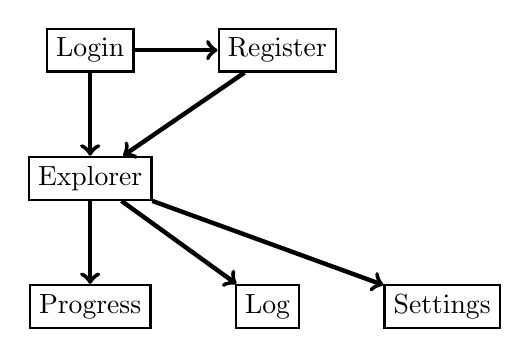
\begin{tikzpicture} [node distance=30pt]
    \node[draw,thick,rectangle] (login) {Login};
    \node[draw,thick,rectangle,right=of login] (register) {Register};
    \node[draw,thick,rectangle,below=of login] (explorer) {Explorer};
    \node[draw,thick,rectangle,below=of explorer] (progress) {Progress};
    \node[draw,thick,rectangle,below=of explorer, right=of progress] (log) {Log};
    \node[draw,thick,rectangle,below=of explorer, right=of log] (setting) {Settings};

    \path (login) edge [->,ultra thick] (register);
    \path (login) edge [->,ultra thick] (explorer);
    \path (register) edge [->,ultra thick] (explorer);
    \path (explorer) edge [->,ultra thick] (progress);
    \path (explorer) edge [->,ultra thick] (log);
    \path (explorer) edge [->,ultra thick] (setting);
\end{tikzpicture}
}\end{figure}
\end{center}
\captionof{figure}{Navigation Flow diagram}
\endgroup

\subsection{Norman’s Design Principles}
Don Norman lists six principles to support software usability. These principles are affordance, constraints, conceptual model, feedback, mapping, and visibility\cite{norman}. The UI decisions for PiSonal trainer comprises of these design principles which are briefly explained below. 
\begin{itemize}
    \item Affordance is the attribute or control that helps the user to determine how it can be used\cite{norman}.
    \item Constraints are the limits of an object or control\cite{norman}.
    \item Conceptual model is a physical understanding of an interaction technique based on real-world experience\cite{norman}. 
    \item Feedback is when the user is provided with information of the results of their actions and directs what actions can be taken next\cite{norman}.   
    \item Mapping is the relationship between a control and its effects\cite{norman}.
    \item Visibility conveys to the user their current state and possible actions\cite{norman}.
\end{itemize}

\subsection{Pages}
\subsubsection{Login}
The login page is the first page that appears when the application is initially opened. It is designed to have strong visibility, such that a new user should know exactly what this page is for and what to do next. There is two empty text fields that indicate user input, and a Login button to proceed. The login button is a constraint as it is disabled until both fields are filled. See Figure 2.

\subsubsection{Register}
The register page is designed similarly to the login page, with strong visibility and a simple and uncluttered design. The empty fields afford input and the register button is disabled until valid input. See Figure 3.

\subsubsection{Explorer}
The explorer page is the main page of the application. From here every other page can be accessed via the navigation bar. The explorer consists of suggested workouts, diet plans, and other interesting articles that may appeal to the user. The buttons within the page affords to be clicked to access the details about that specific section. See Figure 4.
 
\subsubsection{Log}
The log page is used to log specific workouts. This page can be accessed using the navigation bar.  The page layout is similar to the login and register page, where there are empty text fields for user entry and an add button to submit the results to their workout log. See Figure 5 & 6.

\subsubsection{Progress}
The progress page is used to track the user’s workout history. This page can also be accessed using the navigation bar. The progress page consists of charts to visually illustrate the user’s performance as well as a log history below the charts. The there are option buttons the users can choose on how they want to display the data, which acts as the constraints. See Figure 7.

\subsubsection{Settings}
The settings page can be used to logout of the account and also change the user’s profile picture.  This page can also be accessed using the navigation bar. There are two functionality within this page, allowing the page layout to be simple and not cluttered. The buttons on the page aford to be clicked. Feedback is given to the user is they have successfully logged out or changed their picture. 

\begingroup
\begin{center}
\begin{tabular}{| p{5cm} | p{5cm} | p{5cm} |}
    \hline
    \includegraphics[scale=0.50]{login} \captionof{figure}{Login page}& \includegraphics[scale=0.50]{register}\captionof{figure}{Register page screenshot}& \includegraphics[scale=0.50]{explorer}\captionof{figure}{Explore page screenshot} \\
    \hline\\
    \includegraphics[scale=0.50]{log1} \captionof{figure}{Log workout page}& \includegraphics[scale=0.50]{log2}\captionof{figure}{Log workout page screenshot}& \includegraphics[scale=0.50]{progress}\captionof{figure}{Progress page screenshot}\\
    \hline
\end{tabular}
\end{center}
\endgroup

\section{Module Decomposition}
\subsection{Login}   
\fcn
{login (email, password)}
{Email and password to validate user authentication}
{If the response confirms credentials as correct, the user is redirected to the dashboard on the app}
{Allows users to login into their PiSonal Trainer Account using their username/email and password}
\medskip

\subsection{Register}  
\fcn
{signup(email, username, fullname, password, confirm-password)}
{Sends a request to the server with all the fields entered (email, username, fullname, password, confirm password)}
{The response from the server confirms that the account was created, the user is redirected to the login screen of the app and a congratulations alert box is displayed.}
{Allows users to signup for a PiSonal Trainer Account}

\medskip

\subsection{Explorer }  
\fcn
{getWorkoutSuggestions(userid)}
{Sends a request to the server with the userid}
{Respond is an array of suggested workouts, the array is rendered as list view on the Explorer tab page.}
{Provides personalized workout suggestions}

\medskip

\fcn
{getDietSuggestions(userid)}
{Sends a request to the server with the userid}
{Respond is an array of suggested diet plans, the array is rendered as list view on the Explorer tab page.}
{Provides personalized diet suggestions to the user}

\subsection{Progress}   
\fcn
{getLogs(userid)}
{Sends a request to the server with the userid (randomly generated string on signup), to retrieve the user’s workout logs}
{Response is an array of json object with timestamp, exercise name, number of repetitions and sets. This information is rendered as a graph and as a list view of these stats.}
{Gets existing log history}
\medskip

\fcn
{changeGraphView(weeksMode)}
{weeksMode is the input paramater (eg. 1w, 2w, 4w, 8w, 10w, 12w)}
{Changes how many weeks of data is plotted on the graph.}
{Displays graph depending on input type.}
\medskip

\subsection{Log}   
\fcn
{addToLog(userid, exercise, sets, reps, weight)}
{Sends a request to the server with the parameters exercise (String), sets (Integer), reps (Integer), weight (Integer). This adds a log entry/record under the user with userid.}
{Response from the server is a confirmation on whether the addition of a log entry was successfull. If an error message occurs, an error message is displayed and the user is prompted to try again.}
{Add Workout Log}

\subsection{Settings}   
\fcn
{renderSettings()}
{Void}
{Renders the list view of avaliable settings on the Settings tab}
{Renders setting list view}
\medskip

\fcn
{setUserProfileImage(userid, imageURL)}
{Sends the request to the server for setting a new imageURL to the user with userid}
{Response is a confirmation of whether the new imageURL was set for the user with userid}
{Method to set user profile image for account}
\medskip

\fcn
{logout()}
{Void}
{The logged in session on the app is cleared. The cached data (user workout logs) is deleted from the client's device.}
{Method to logout of user account}

\subsection{Counting algorithm}
%Object detection and tracking is performed using OpenCV with a Macbook webcam. The algorithm for counting repetitions and sets is implemented in Python.
\fcn
{cameraLoop(camera, pts, reps)}
{A reference to the camera, position values of the object over time, number of reps}
{Void}
{Continuously checks motion detected by the camera to determine if a rep has been performed, or if the set has ended.}
\medskip

\fcn 
{detectDirection(prev, cur, reps)}
{Previous position, current position, rep count}
{Updated rep count}
{Updates the reps variable, which keeps count of the number of repetitions of a movement. It uses slopes to determine whether the object is moving upwards (positive) or downwards (negative). A consecutive up and down movement counts as one rep.}
\medskip 

\fcn 
{detectEndOfSet(stop0, t0, sets, reps)}
{Time when object stopped, current time, set count, rep count}
{Updated values of stop0, sets and reps}
{Detects the end of a set if object stays in the same area for more than 10 seconds. The object does not need to stay perfectly still as the average of the last 3 position values of the object is compared to an offset value.}

\newpage

\section{Relational Database Structure}
\subsection{ER Diagram}

\begingroup
\begin{center}
\begin{figure}[h]
\center{
\begin{tikzpicture} [node distance=30pt]
     
     
    \node[draw,thick,ellipse, below=of email] (reps) {reps};
    \node[draw,thick,rectangle, below=of reps] (log) {Log};
    \node[draw,thick,ellipse,below=of log] (uid) {\underline{userid}};
    \node[draw,thick,ellipse,below=of password, left=of reps] (exrName) {exerciseName};
    \node[draw,thick,ellipse,below=of log, left=of uid] (sets) {sets};
    \node[draw,thick,ellipse,below=of log, left=of sets] (time) {timeStamp};
    \node[draw,thick,ellipse,above=of time] (weight) {weight};
     
    \node[draw,thick,diamond,right=of log] (logs) {logs};
    
    \node[draw,thick,rectangle, right=of logs] (users) {Users};
    \node[draw,thick,ellipse,below=of users] (id) {\underline{userid}};
    \node[draw,thick,ellipse, right=of users] (userName) {username};
    \node[draw,thick,ellipse,below=of userName] (email) {email};
    \node[draw,thick,ellipse,above=of users] (password) {password};
     
    \path (users) edge [->,ultra thick] (id);
    \path (users) edge [->,ultra thick] (userName);
    \path (users) edge [->,ultra thick] (email);
    \path (users) edge [->,ultra thick] (password);
    
    \path (users) edge [-,ultra thick] (logs);
    \path (logs) edge [->,ultra thick] (log);
    
    
    \path (log) edge [->,ultra thick] (uid);
    \path (log) edge [->,ultra thick] (exrName);
    \path (log) edge [->,ultra thick] (time);
    \path (log) edge [->,ultra thick] (reps);
    \path (log) edge [->,ultra thick] (sets);
    \path (log) edge [->,ultra thick] (weight);
\end{tikzpicture}
}\end{figure}
\end{center}
\captionof{figure}{ER diagram PiSonal Trainer table descriptions}
\endgroup

\subsection{Table Descriptions}
\begin{itemize}
    \item \textbf{Users} table stores users' credentials and basic information.
    \item \textbf{Logs} table contains all the records for every user, identified by the userid.
\end{itemize}

\section{Development Details}
\begin{itemize}
    \item Languages of implementation
    \begin{itemize}
        \item Objective-C
        \item JavaScript
    \end{itemize}
    \item Supporting frameworks
    \begin{itemize}
        \item OpenCV
        \item React Native
    \end{itemize}
    \item Supporting technology
    \begin{itemize}
        \item Camera on iOS devices
    \end{itemize}
\end{itemize}


\begin{thebibliography}{9}
\bibitem{norman} 
Norman, D. The Design of Everyday Things. Basic
Books, New York, 2013.
\end{thebibliography}

%%%%%%%%%%%%%%%%%%%%%%%%%%%%%%%%%%%%%%%%%%%%%%%%%%%
% REFERENCES
%%%%%%%%%%%%%%%%%%%%%%%%%%%%%%%%%%%%%%%%%%%%%%%%%%%
% \section*{References}

%%%%%%%%%%%%%%%%%%%%%%%%%%%%%%%%%%%%%%%%%%%%%%%%%%%
% INDEX
%%%%%%%%%%%%%%%%%%%%%%%%%%%%%%%%%%%%%%%%%%%%%%%%%%%
%\section*{Index}

\end{document}

The document should include the system architecture design and component design. You should give the architecture of the system, system components, APIs, algorithms used, solutions to address the challenges mentioned in your previous report, and shows the reasons on your design choices.
Contact GitHub API Training Shop Blog About
© 2017 GitHub, Inc. Terms Privacy Security Status Help